%# -*- coding: utf-8-unix -*-
%%==================================================
%% chapter01.tex for SJTU Master Thesis
%%==================================================

\chapter{绪论}
\label{chap:intro}

\section{论文研究的背景及意义}
\label{sec:intro:analog}
	20 世纪以来,人类生存环境中化学品日益增多,对数量巨大且种类复杂的
	化学物进行健康风险的评估是公共健康领域当前重要的研究课题。此外,人类与
	环境化合物的接触方式多为低剂量下的复合暴露,如何实现高通量的毒性评价和
	科学的风险评估成为研究的热点与难点。
	
		自 2005 年起,美国启动了 21 世纪毒理学研究计划(TOX21),主要借助体
	外测试和计算生物信息学等方法进行高通量化学品毒性评估。然而,使用细胞或
	类器官的体外方法虽然可以进行较高通量的毒性测试,但无法代替动物体内实
	验,因为其结果无法反映化合物进入生物体内吸收、分布、代谢与排泄环节对毒
	性的影响。传统的动物体内毒性研究结果具有很大的参考意义,但是实验周期长、
	成本高,并且涉及动物保护与伦理。如果进行待测化合物低剂量复合暴露毒性研
	究,需要不同化合物的多剂量进行配伍,基于上述动物实验的局限性,难以进行
	高通量的毒性测试。秀丽隐杆线虫作为一种模式生物,对环境变化非常敏感;其
	生命周期和寿命较短,身体尺寸较小易操作,以大肠杆菌为食易培养,身体透明
	易观察,染色体和基因组较小易分析,生物学信号通路保守,因此近年来线虫被
	广泛应用于重金属、PM2.5、农药、纳米颗粒和有机污染物等环境毒理学研究领
	域。国际上目前已进展到第三阶段的 TOX21 计划也在使用包括线虫在内的模式生
	物对前期结果进行验证,并计划对更多环境化合物进行毒性筛选。
	
		传统的线虫培养方法在液体或琼脂板上进行,需要的线虫数量多,待测化合
	物所需量较大,此外难以对单个线虫实现精确刺激、操控和追踪。微流控体系与
	线虫大小尺度相匹配,有望实现线虫芯片内培养、成像和数据分析等。自从 2011
	年美国启动“类器官芯片”计划之后,以微流控芯片为平台的毒理测试技术发展
	迅速,相比器官芯片平台,线虫芯片是在动物个体水平上进行毒理学研究,具有
	不可替代的优势。
	
\section{秀丽隐杆线虫概述}
	\begin{figure}[h]
	  \centering
	  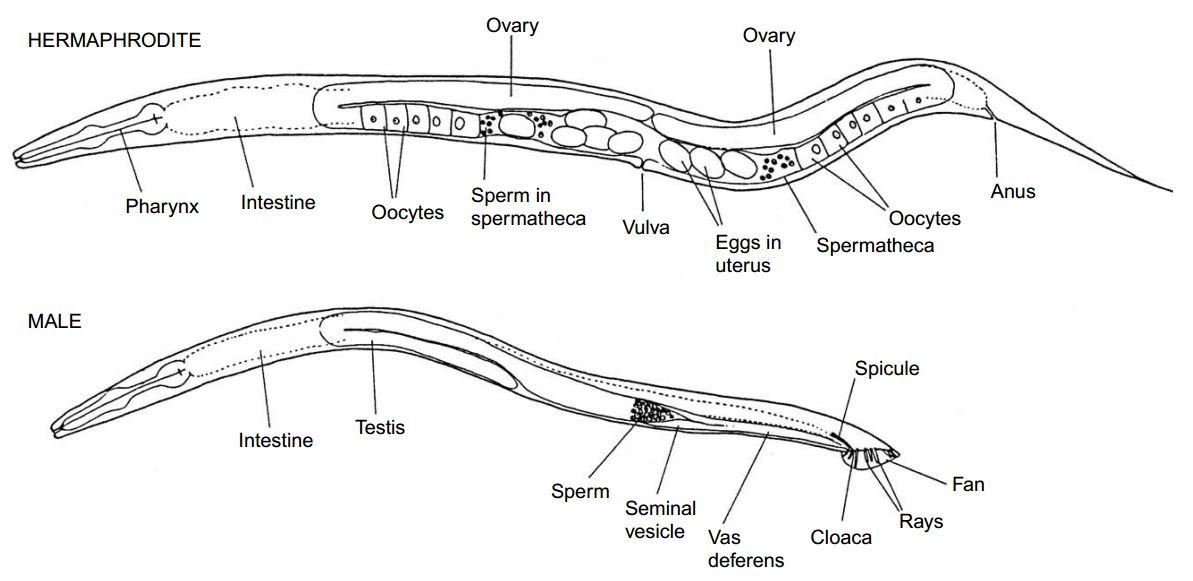
\includegraphics[width=14cm]{figure/chap1/Celegans.jpg}
	  % \hspace{1cm}
	  % 
\includegraphics[width=4cm]{example/sjtulogo.jpg}
	  \bicaption[这里将出现在插图索引中]
		{秀丽隐杆线虫解剖图}
		{Anatomy of adult C.elegans.}
	  \label{fig:Celegans}
	\end{figure}
	秀丽隐杆线虫(简称 C. elegans)是一种微米尺度的无脊椎模式生物,主要生活在土壤中或水中,以大肠杆菌OP50为食,成虫
	体长约为1mm宽度50um,并且从幼虫长到成虫只需要3天。秀丽隐杆线虫是线虫动物门中的一种,包含雌雄同体和雄性两种性别如图\ref{fig:Celegans}。两种性别都是二倍体,都有五对常染色体,
	但雌雄通体的线虫有两个X常染色体(XX)而雄性线虫只有一个X常染色体(XO)。在自然条件下,线虫几乎都为雌雄同体,
	雄性个体只占约五百分之一。线虫的生命周期较为简单如图\ref{fig:lifecycle}所示,成年雌雄同体线虫同时含有精子和卵母细胞,因此能够自体受精。
	每一个自体受精的雌雄同体线虫大约可以产生330多个蛋。如果雄性体线虫交配产蛋量将会提高,并且有利于
	基因的重新组合。在25$^。C$下孵化12个小时即可得到L1期的线虫幼虫,
	长度约为0.15mm。L1期幼虫基本上具备了和成虫一样的器官结构,除了还没有形成生殖器结构,从L1期线虫
	长到L4期只需要3天。
	线虫作为一种现代动物模型被广泛地用于细胞生物学、神经科学、衰老与发育和毒理学等研究中。在2002年
	,研究秀丽线虫的研究团体就已经扩展到300多个实验室,分布在20多个国家和地区。1998年,构成整个基因组的9700万个碱基对DNA的测序基本完成,
	这是第一个经过完整基因组测序的多细胞生物。与其他模式生物相比线虫具有如下技术优势:
	
	\begin{itemize}
	  \item 由于线虫通体透明,可以通过荧光蛋白标记的表达观察细胞的分裂等许多重要的生理过程,
	  还可以用于对神经元成像,研究外部刺激与神经元活动之间的关联。
	  \item 线虫的生命周期短、培养简单以及繁殖能力强,这些特性都有助于加快实验周期,提高实验的并行性。
	  \item 线虫身体构造简单,遗传模式保守,有利于减小实验中由于个体差异而引起实验结果的扰动。
	  \item 对线虫基因的测序已经完成,使得线虫可以在基因筛查分析和其他遗传学实验中发挥重要作用。
	  \item 线虫基因与人类的基因有约40\%的同源性,许多的研究者将线虫作为疾病模型研究疾病机制。
	\end{itemize}
	

	\begin{figure}[h]
	  \centering
	  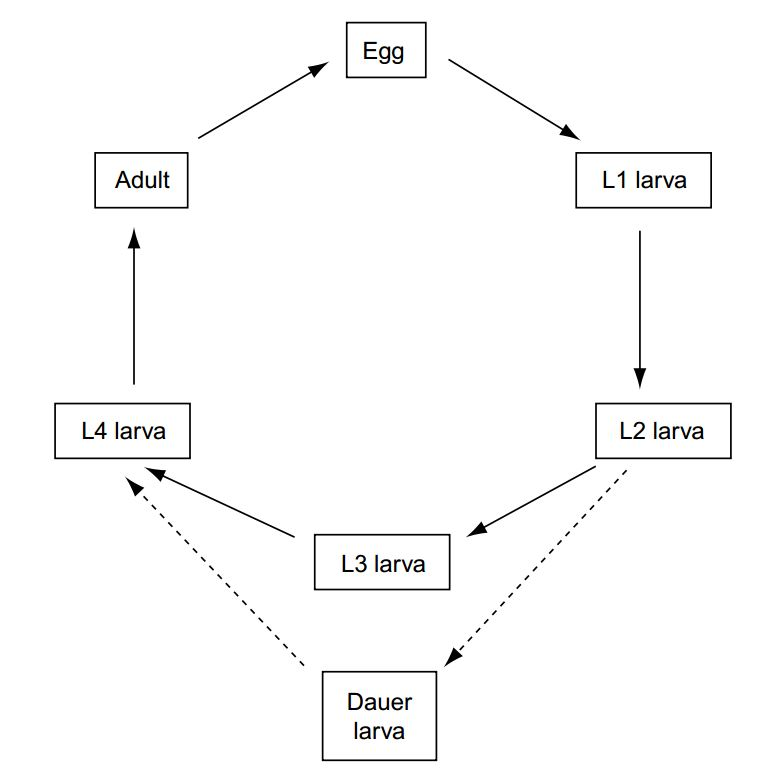
\includegraphics[width=8cm]{figure/chap1/lifecycle.jpg}
	  % \hspace{1cm}
	  % 
\includegraphics[width=4cm]{example/sjtulogo.jpg}
	  \bicaption[这里将出现在插图索引中]
		{秀丽隐杆线虫生命周期}
		{The life cycle of C.elegans.}
	  \label{fig:lifecycle}
	\end{figure}
	
\section{国内外研究现状}
\label{sec:intro:analog}
	微流控是一种在微米尺度操纵流体的技术,具有反应体系小、通量高、自动化且操作灵活等优势,被越来越多的应用于细胞和微米尺度生物的研究中。
	微流控技术在线虫研究中的应用为研究者们提供了一个全新的研究平台,极大的促进了相关领域的研究进展。利用微流控技术研究线虫具有的
	优势有:\begin{enumerate*}[label=\itshape\alph*)\upshape]
	\item 利用微流控芯片可以实现在细胞尺度上对线虫的操纵。\quad
	\item 利用微流控芯片可以实现对线虫的快速固定与成像,与使用药物麻醉的方法相比,这种固定
		方式不会对线虫产生任何损害,线虫可以在后续步骤中恢复。\quad
	\item 利用微流芯片可以快速的从上千只线虫中的筛选出需要的表型,实现线虫的分选。\quad
	\item 微流控芯片可以为线虫的培养提供精确的微环境,为线虫的感知实验提供精确的刺激传达。\quad
\end{enumerate*}
	本文将从以下几个方面对近年来国内外相关领域的发展状况进行回顾,包括线虫的分选、线虫固定与成像以及介绍微流控在毒理学实验中的研究进展。
	最后介绍近年来线虫图像处理的研究进展。
	
\subsection{微流控芯片线虫操控方法}
	在线虫的实验中,经常涉及一些对线虫的日常操纵。如线虫的片上培养、线虫分选、线虫的固定与成像等。
	为了避免复杂的人工操作,研究者们提出了许多不同用途的芯片,这些芯片能够将不同的操作集成在一起,极大的
	提高了实验的并行性和自动化程度。
	
\subsubsection{线虫的培养}
\label{sec:intro:analog}
	线虫的长期培养是研究线虫的衰老和发育的基础,在许多需要对线虫进行长期观察的实验中也需要解决线虫的长期培养问题。
	线虫的长期培养需要与外部环境进行物质交换,包括氧气和食物的供应以及将废物排出。微流控芯片的制作材料一般为聚二甲基硅氧烷
	(ploydimethylsiloxane, PDMS),这种材料具有很好的透气性,因此微流控芯片可以为线虫提供氧气。其中一个早期的工作是由Kim等人\cite{Kim2007Automated}
	完成的,他们设计了一款类似于CD形状的微流控芯片可以实现线虫的片上培养长达数天。食物会在离心力的作用下进入到线虫的培养腔室。
	线虫腔室中的废物会在离心力的作用下被甩出,从而实现了物质的交换。这款芯片可以将线虫培养到三代并且不会影响到线虫的
	生长和行为。然而,由于其芯片结构设计较为简单,所以无法区分不同代之间的线虫且不能实现对单个线虫的跟踪和
	成像。
	\begin{figure}[h]
	  \centering
	  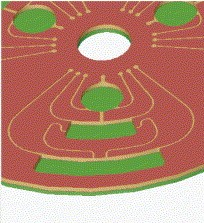
\includegraphics[width=8cm]{figure/chap1/cd.jpg}
	  \bicaption[这里将出现在插图索引中]
		{CD状线虫培养芯片}
		{The life cycle of C.elegans.}
	  \label{fig:cd}
	\end{figure}
	
	由于以上的局限,Hulme等\cite{Hulme2010Lifespan}设计了一款新的芯片。由一排平行的腔室组成,可以实现线虫
	的长期培养及研究其运动行为。利用侧边的楔形通道来固定线虫可以实现线虫的固定与成像以及监测其体长的变化。
	可以同时培养16条成虫,极大的加快了衰老相关的研究,并发现线虫的摆动频率会随着线虫发育日渐成熟而出现下降。
	另一方面,研究者们将液滴和可逆凝胶运用在线虫的长期培养中\cite{Aubry2015Hydrogel,Krajniak2010Long,Wen2015A,Cornaglia2016Automated}。
	Krajniak 和 Lu\cite{Krajniak2010Long}开发了一款集成微流控芯片,该芯片由8个微腔室构成,通过周围的微管道和阀门控制。成功地
	展示了在一块芯片上进行线虫地培养、固定与成像等操作。线虫由一个入口通道进入到8个线虫培养腔室,并将PF127
	可逆凝胶经入口通道注入到线虫培养腔室。这种聚合物在低温(大约15$^\circ$C)下呈现较高地粘性,
	在高温下(大约21$^\circ$C)呈现胶状。运用这款芯片,成功实现了从L1期线虫到成虫过程的生理监测。
\subsubsection{线虫的固定}
\label{sec:intro:analog}
	线虫的固定对于线虫神经元成像与显微手术\cite{Gokce2014A}等需要固定线虫的实验是至关重要的。传统的线虫固定方法经常使用胶水或者麻醉剂
	来固定线虫,使用胶水固定线虫往往很难在短时间内恢复,而使用麻醉剂对线虫神经元可能产生潜在的影响。因此,为了
	实现可逆的无损伤的固定线虫,研究者提出很多基于微流控固定线虫的方法。Chokshi等人\cite{Chokshi2009CO2}开发了一款简单的
	微流控芯片可以有效的固定线虫,并运用这款芯片研究了线虫的运动行为。作者比较了两种不同的固定方法,第一种方法是在上层
	PDMS通道中通入二氧化碳,利用PDMS材料的透气性,上层二氧化碳会向下层扩散从而达到固定线虫的目的;第二种方法是在上层通道
	中施加一个大的气压,从而使中间的PDMS模形变,从而可以将线虫固定。作者还通过评估线虫的运动速度来量化两种不同的固定方式
	对线虫产生的影响,他们发现通过二氧化碳方法固定线虫比用机械的方法固定对线虫的影响较小。
	
	以上的方法虽然能够对成虫进行固定,但由于幼虫的尺寸比成虫小且L1期的幼虫很容易
	将微通道阻塞,因此幼虫的固定是个难点。Aubry等人\cite{Aubry2015Hydrogel}运用FP127凝胶液滴将L1的幼虫包裹,当液滴进入到存储单元
	时可以调整温度从而固定线虫,成功实现对L1期幼虫的操纵及成像。为了研究线虫胚胎发育及其分子机制,Cornaglia
	等人\cite{Cornaglia2015An}设计了一款可以固定线虫胚胎并对其成像的微流控芯片。其由一个线虫培养腔室和许多个微小的胚胎腔室阵列组成,
	研究者可以在胚胎腔室中固定线虫胚胎并且实时观察胚胎发育的整个过程,这种阵列式的腔室结构支持同时对多个线虫
	胚胎进行观察,具有高通量的优势。还有一些研究者利用狭窄的微通道来固定线虫\cite{Lee2014A,Hulme2007A},通过对线虫的存活率和子代的数目
	进行统计发现这种固定方式对线虫没有产生明显影响。
\subsubsection{线虫的分选}
\label{sec:intro:analog}
	目前,使用正向和反向基因筛查的方式筛选新的基因是理解分子通路和蛋白功能的一种非常有效的方法。而在成百上千
	的线虫中筛选出特定表型的线虫是一件耗时且工作量很大的事情,运用微流控器件可以极大的缩短筛查的时间并可以很快
	对观察到的基因变种进行分选。线虫分选芯片的操作往往是基于线虫某种表型的特性如趋电性、行为表型、尺寸、
	运动能力以及电生理学特性的不同等。Rezai\cite{Rezai2012Electrical}等人利用线虫的趋电性设计了一种单层微流控芯片,可以有效的分选出不同
	发育阶段的线虫以及具有神经缺陷的变种。Casadevall\cite{Casadevall2011High}等人设计了一款芯片可以对不同尺寸的线虫同步化,并且可以实现
	每分钟200-1200条线虫的分选速率。Dong\cite{dong2016versatile}等人设计了一种双层的基于PDMS膜形变的线虫分选芯片。通过控制上层气压使
	下层流道层的尺寸发生改变从而只允许特定尺寸的线虫通过这些通道进入另一个腔室。这种方法需要对特定尺寸的线虫
	精确控制施加气压的大小,这款芯片可以以每秒3.5个线虫的速率进行分选。
	% \label{sec:intro:analog}
	% 
	% 可从以下角度分类。
	% \begin{itemize}
	  % \item 有许多文献基于线虫的大小从而对幼虫和成虫进行分选。
	  % \item 线虫的趋电性的不同导致线虫向不同的电极靠近从而达到分选的目的,文献若干。
	  % \item 基于神经元活动和电生理特性的筛选。
	  % \item 区别于物理固定和可逆凝胶固定线虫,研究者提出了一种将液滴捕获用于线虫的分选。
	% \end{itemize}

\subsection{药物筛选与毒理实验}
\label{sec:intro:analog}
	线虫作为一种重要的模式生物与人类的疾病基因具有约65\%的相似性\cite{Baumeister2002The,Sonnhammer1997Analysis},
	因此线虫在药物筛选和毒理学研究领域经常作为一种重要的研究对象。近年来,研究者们设计了很多用于实时药物
	识别、筛选和毒性测试的微流控芯片。Chung等人\cite{Chung2011Microfluidic}开发了一款包含48个平行阵列腔室的微流控芯片,每一个腔室单元的
	直径为1.5mm,并且还设计了一条宽500um的管道用于将线虫和化合物送到每个腔室。所有的腔室在视野种都是可见的,因此
	便于观察每个腔室中单个线虫暴露在某种化合物下的反应。Yang等人\cite{Yang2013An}开发了一款双层的可以评估体内抗菌活性的微流控芯片,
	芯片呈现放射状四周分布着32个腔室,中心有一个存储的腔室,有四个“圣诞树”结构的片上浓度梯度生成器\cite{Dertinger2001Generation,Jeon2000Generation}。利用
	这款芯片可以同时研究4种药物32种浓度梯度对线虫的影响。中科院大连化学物理研究所设计制作了一种三夹层的芯片,
	该芯片由上层液路层、中间气路控制层和底层玻璃组成。液路层有30个长2mm$\times$宽1mm$\times$厚70um的线虫
	培养腔室用于线虫培养何成像,中间有一个废液池用于收集线虫培养腔室中的废液。并应用该芯片探究了高糖对线虫
	寿命的影响\cite{zhuliguo2016}。
	% 很多的线虫芯片被开发,用于药物识别,筛选、以及研究毒性对线虫行为、生理电信号衰老。抗菌和代谢
% 活动身体毒性的影响。
	% \begin{itemize}
	  % \item 多种复合药物浓度梯度的药物筛选。
	  % \item 将线虫暴露在细菌病原体环境中。
	  % \item 将线虫暴露在重金属环境中
	% \end{itemize}
	
\subsection{机器视觉在线虫研究中的应用}
\label{sec:intro:analog}
	研究线虫的运动行为并对其量化在许多线虫研究中(如:神经学、遗传学和毒理学等研究中)起着十分重要的作用,
	通过人工观察不仅效率低下而且还会引入人为误差,如在基因筛查中需要在成百上千的线虫发现行为异常的线虫往往
	需要分析几百个小时的视频,因此应用机器视觉的方法量化运动相关的表型具有重要的意义。近年来,研究者们提出
	很多自动化线虫图像处理的方法。Dhawan等人\cite{De1998Natural}设计一个可以在较低的倍率同时跟踪多个线虫的系统,
	但是该系统只能得到线虫运动方向等信息,无法得到线虫形态和姿势等相关特征(如体长、运动速度等)。
	Baek等人\cite{Baek2002Using}开发了一个可以在较高倍率下跟踪单个线虫的系统,通过控制载物台的移动可以
	保证线虫始终出现在视野中,通过提取94种不同的特征并利用决策树对特征向量进行分类可以区分出行为异常的线虫变种。
	在2011年,剑桥大学分子生物学实验室研究人员设计了一款名为Wormtracker的系统,该软件可以包含一套定制的软硬件
	系统\cite{yemini2013high}。与之前的单线虫跟踪系统相比,可以将成本下降四分之一,该系统另一个优点是能够实现对所有发育阶段的幼虫
	的跟踪以及游动状态下单线虫的跟踪。Swierczek等人\cite{swierczek2011high}设计了一款名为
	Multi-Worm Tracker(MWT)的软件,最多可以实现对120条线虫的跟踪,但只能以离线的方式对采集到的
	视频数据进行特征提取无法实现特征的实时提取。另外,当多个线虫的相遇并相互遮挡时,系统只会识别到一个轮廓,
	这样会导致跟踪的失败。
	
	为了解决线虫跟踪过程中线虫轮廓的重叠与遮挡的问题,研究者们提出了一些基于模型的跟踪算法。Restif等人\cite{restif2008tracking}
	提出一种针对游动线虫的跟踪算法。其将线虫的跟踪分成两个阶段:第一个阶段是通过线虫轮廓运动的历史状态预测下个状态
	线虫轮廓运动的速度,结合当前状态下线虫轮廓的位置可以计算出下个时刻线虫轮廓出现的位置;第二个阶段主要是
	调整上个阶段得到的线虫轮廓使其与图片上线虫的轮廓重合。 Fontaine和Roussel等人\cite{fontaine2007model,roussel2014robust}提出了一种
	可以对线虫和斑马鱼进行跟踪的算法,其主要思想是通过对线虫轮廓进行参数化建模得到状态空间并通过
	迭代卡尔曼滤波器来预测模型参数从而实现线虫的跟踪。针对单个线虫发生自身卷曲时其轮廓识别的困难,Nagy等人
	\cite{nagy2015generative}提出一种基于统计生成式方法可以识别复杂的姿态。
	
	线虫的图像处理一般分为两个模块,分别是线虫的跟踪(包括线虫轮廓的分割)和线虫的特征提取。线虫的跟踪模块
	主要是得到线虫的轮廓,线虫的特征提取模块是利用跟踪到的线虫轮廓进行特征计算。Yemini等人\cite{yemini2013database}
	对线虫相关的行为表型进行了综述并将其分为四大类:分别为形态特征(如:体长、体宽和面积等)、姿势特征(如:
	线虫脊线的水平投影长度、波长以及弯曲的数量等)、运动特征(如:运动速度和运动状态等)、轨迹特征(如:线虫重心
	移动轨迹的范围和轨迹图等)。线虫姿态的描述一般是通过在线虫的中间脊线上等距的采样固定数量的点来定义的。
	这样得到线虫姿势的状态空间通常是很大的,Stephens等人\cite{Stephens2008Dimensionality}提出一种降维的方法
	从而可以在较低的维度空间描述线虫的姿势状态。其主要的思想是计算线虫中间脊线的曲率从而得到一个曲率向量,
	并对其归一化然后计算这个向量的协方差矩阵,发现其大部分的特征值为零。作者取了四个最大的特征值对应的
	特征向量作为四个本征向量,这四个本征向量将构成一个状态空间,任何线虫脊线曲率向量都可以投影到这个空间。
	由此得到四个投影长度即可描述线虫的姿势。即可以在一个四维空间中描述线虫的姿势。Restif等人\cite{Restif2014CeleST}提出了一种新的
	计算特征的方法。通过将计算同一个线虫的脊线曲率向量并将其按照时间顺序排列,由此即可得到一个矩阵。通过
	对这个矩阵做二维离散傅里叶变换。最后基于傅里叶变换的结果计算线虫相关的特征。为了实现线虫行为数据的
	共享,Javer等人\cite{Javer2018An}提出统一的数据格式支持对视频数据以及对应的特征数据的读取以存储。
	并定义了一种中间数据格式表示Worm tracker Commons Object Notation (WCON)这样可以方便研究者组合使用不同
	线虫跟踪模块和特征提取模块。
\section{存在的问题}
\label{sec:intro:analog}
	\begin{itemize}
	  \item 片上梯度的形成
	  \item 游动线虫轮廓的分割
	  \item 一个集成微流控芯片和多线虫实时图像处理的平台还报道的比较少
	\end{itemize}
\section{研究内容}
\label{sec:intro:org}
	\begin{itemize}
	  \item 首先搭建了一个基于微流控芯片的硬件平台
	  \item 设计了一款及线虫轮廓分割、跟踪及特征提取等功能的自动化图像处理软件。
	  并针对线虫分割的鲁棒性与实时性的要求,还提出了一种基于深度学习的线虫轮廓分割的网络。
	  \item 在搭建的硬件平台上,并通过双氧水实验验证 系统的优势。
	\end{itemize}
\section{论文章节安排}
\label{sec:intro:org}
